\usetikzlibrary{fit, positioning}

\section{Directed graphical models (Bayes nets)}

\exercise[]{
\textbf{Consider the DAG in Figure 10.14(a). Construct a new DAG where you
marginalize out $X$.}

The important thing to note here is that while conditioning a variable acts
like a ``blocker" node, marginalizing a node does the opposite. It removes
the node from the DAG, and adjusts all nodes accordingly.

To illustrate some properties of marginalization, let a shaded node mean a
marginalized node. In this case

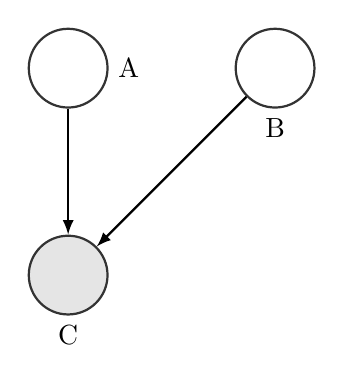
\begin{tikzpicture}
\tikzstyle{main}=[circle, minimum size=10mm, thick, draw=black!80, node distance=16mm]
\tikzstyle{connect}=[-latex, thick]
\tikzstyle{box}=[rectangle, draw=black!100]
    \node[main, fill = white!100] (A) [label=right:A] { };
    \node[main, fill = white!100] (B) [right=of A, label=below:B] { };
    \node[main, fill = black!10]  (C) [below=of A, label=below:C] { };
    \path (A) edge [connect] (C)
          (B) edge [connect] (C);
\end{tikzpicture}

Node C is marginalized and this DAG reduces to

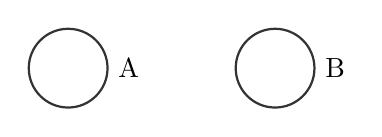
\begin{tikzpicture}
\tikzstyle{main}=[circle, minimum size=10mm, thick, draw=black!80, node distance=16mm]
\tikzstyle{connect}=[-latex, thick]
\tikzstyle{box}=[rectangle, draw=black!100]
    \node[main, fill = white!100] (A) [label=right:A] { };
    \node[main, fill = white!100] (B) [right=of A, label=right:B] { };
\end{tikzpicture}

In other words, since A and B are parents of C, marginalizing on C will make A
and B independent of each other. Another situation is

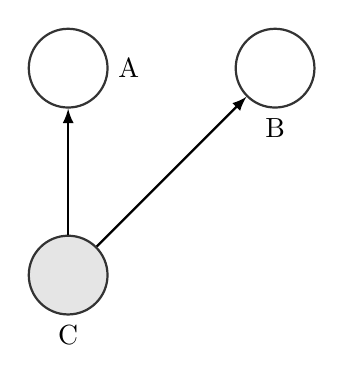
\begin{tikzpicture}
\tikzstyle{main}=[circle, minimum size=10mm, thick, draw=black!80, node distance=16mm]
\tikzstyle{connect}=[-latex, thick]
\tikzstyle{box}=[rectangle, draw=black!100]
    \node[main, fill = white!100] (A) [label=right:A] { };
    \node[main, fill = white!100] (B) [right=of A, label=below:B] { };
    \node[main, fill = black!10]  (C) [below=of A, label=below:C] { };
    \path (C) edge [connect] (A)
          (C) edge [connect] (B);
\end{tikzpicture}

Node C is marginalized and this DAG reduces to

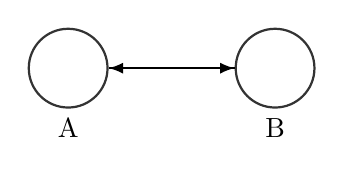
\begin{tikzpicture}
\tikzstyle{main}=[circle, minimum size=10mm, thick, draw=black!80, node distance=16mm]
\tikzstyle{connect}=[-latex, thick]
\tikzstyle{box}=[rectangle, draw=black!100]
    \node[main, fill = white!100] (A) [label=below:A] { };
    \node[main, fill = white!100] (B) [right=of A, label=below:B] { };
    \path (A) edge [connect] (B)
          (B) edge [connect] (A);
\end{tikzpicture}

In this situation, C is a parent of A and B. Marginalizing out C causes and A
and B to be dependent to each other.

Applying these rules to the DAG in the problem text, we note that node X is
both a child and a parent node. By marginalizing X, it removes the dependence
on A and B, but adds dependencies to A and B through the children of X. In
other words, by removing X, now A and B influence E and F. Particularly,
both A and B influence both E and F. The DAG then looks like

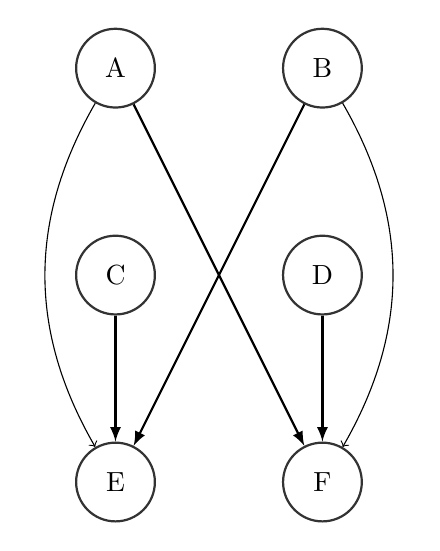
\begin{tikzpicture}
\tikzstyle{main}=[circle, minimum size=10mm, thick, draw=black!80, node distance=16mm]
\tikzstyle{connect}=[-latex, thick]
\tikzstyle{box}=[rectangle, draw=black!100]
    \node[main, fill = white!100] (C) [] {C};
    \node[main, fill = white!100] (E) [below=of C] {E};
    \node[main, fill = white!100] (D) [right=of C] {D};
    \node[main, fill = white!100] (F) [below=of D] {F};
    \node[main, fill = white!100] (A) [above=of C] {A};
    \node[main, fill = white!100] (B) [above=of D] {B};
    \path (A) edge [connect] (F)
          (B) edge [connect] (E)
          (C) edge [connect] (E)
          (D) edge [connect] (F);
    \draw[bend right, ->] (A) to node [auto] {} (E);
    \draw[bend left, ->]  (B) to node [auto] {} (F);
\end{tikzpicture}

As you can see, both nodes A and B now affect E and F.

}

\exercise[]{
\textbf{Bayes ball. \\
a. Consider the DAG in Figure 10.14(b). List all variables that independent of
A given evidence on B.}

``Given evidence on B" is another way of saying ``conditional on B". To find
all of the variables that are independent of A, we look at all the paths that
each variable can arrive at A through, and examine them with the knowledge
of B.

Let's go through the nodes then.

Node C: this node is a parent of A, and thus is not independent of A, even
knowing B.

Node D: from node D, we can reach A through $\{D,B,A\}$, $\{D,G,E,C,A\}$, and
$\{D,G,I,H,C,A\}$. Conditioning on B blocks $\{D,B,A\}$, but not the others.
Therefore, D is not independent of A, conditioned on B.

Node E: we can reach node A using $\{E,C,A\}$, which is unblocked. Therefore
node E is not independent of node A.

Node F: we can reach node A using $\{F,C,A\}$, which is unblocked. Therefore
node F is not independent of node A.

Node G: we can reach node A using $\{G,E,C,A\}$, $\{G,D,B,A\}$, or
$\{G,I,H,F,C,A\}$. The path $\{G,D,B,A\}$ is blocked, but the others are not,
and therefore node G is reachable from node A.

Node H: we can reach node A using $\{H,F,C,A\}$, $\{H,I,G,E,C,A\}$, or
$\{H,I,G,D,B,A\}$. The path $\{H,I,G,D,B,A\}$ is blocked, but the others are
not, and therefore node H is reachable from node A.

Node I: we can reach node A using $\{I,H,F,C,A\}$, $\{I,G,D,B,A\}$, or
$\{I,G,E,C,A\}$. The path $\{I,G,D,B,A\}$ is blocked, but the others are not,
and therefore node I is reachable from node A.

Thus, the only node that is independent to A conditioning on B is B.

\textbf{b. Consider the DAG in Figure 10.14(c). List all variables that are
independent of A given evidence on J.}

Note that since G is the sole parent of J and J has no children, conditioning
on J is equivalent to conditioning on G.

Next, let's identify the hidden nodes. These are $\{H,I\}$. This means that
nodes ${C,F}$ are blocked from the rest of the DAG and are independent of A.

For the remaining nodes, note that conditioning on G opens up paths to A,
since all paths to A from other nodes that go through G will go through a
v-structure node. Thus, nodes $\{B,D,E\}$ are all not independent of A.

Thus, nodes $\{G,J,H,I,C,F\}$ are all independent of A after conditiong on J.

}

\exercise[]{
\textbf{Markov blanked for a DGM.}

We want to prove that the conditional for a node is given by the conditional
of the node with its parents times the conditional of its children with itself.
The conditional is given by

\begin{align}
    p(X_i|X_{-i}) & = \frac{p(X_{-i}|X_i)p(X_i)}{p(X_{-i})} \\
    & = \frac{p(X_i) \prod_{t \neq i}^T p(X_t|pa(X_t),X_i)}
             {\prod_{t \neq i}^T p(X_t|pa(X_t))}
\end{align}

Note that for the children $X_c$ of $X_i$, $pa(X_c) = X_i$. Thus, the numerator
becomes

\begin{align}
    p(X_i|X_{-i}) = \frac{p(X_i) \prod_{Y_j \in ch(X_i)} p(Y_j|pa(Y_j))
                                 \prod_{t \neq i}^T p(X_t|pa(X_t),X_i)}
                         {\prod_{t \neq i}^T p(X_t|pa(X_t))}
\end{align}

Note that Equation 10.7 comes in handy here. it says that
$p(X_{1:V}) = \prod_{t=1}^V p(x_t|pa(x_t))$. What follows from this is that
nodes are not affected by nodes that aren't its parents. Thus, we can write
this quantity as

\begin{align}
    p(X_i|X_{-i}) & = \frac{p(X_i|pa(X_i))\prod_{Y_j \in ch(X_i)}p(Y_j|pa(Y_j))
                                 \prod_{t \neq i}^T p(X_t|pa(X_t))}
                         {\prod_{t \neq i}^T p(X_t|pa(X_t))} \\
                  & = p(X_i|pa(X_i))\prod_{Y_j \in ch(X_i)}p(Y_j|pa(Y_j))
\end{align}

}

\exercise[]{
\textbf{Hidden variables in DGMs. \\
a. Assuming all nodes (including H) are binary and all CPDs are tabular,
prove that the model on the left has 17 free parameters.}

In general, a variable with $K$ states have $K-1$ free parameters. So, binary
variables will have $1$ free parameter. Thus $p(X_i)$ has $1$ free parameter.

We can write $P(X_n|X_{n-1},...,X_1)$ as
$P(X_n=n|X_{n-1}=m,...,X_1=a) = T_{nm...a}$. Since we are dealing with binary
variables, we note that $T_{nm...a}$ is indexed with a binary string of length
$n$. The number of states in a binary string of length $n$ is $2^{n-1}$. Thus,
$P(X_n|X_{n-1},...,X_1)$ has $2^{n-1}$ free parameters.

The joint distribution of this particular DGM is given by

\begin{align}
    p(X_{1:6}) & = p(X_1)p(X_2)p(X_3)\sum_h p(H=h|X_{1:3})p(X_4|H=h)
                   p(X_5|H=h)p(X_6|H=h)
\end{align}

Going left to right from each term in the joint, the number of free parameters
are given by

$$1 + 1 + 1 + 2^3 + 2 + 2 + 2 = 17$$

\textbf{b. Assuming all nodes are binary and all CPDs are tabular, prove that
the model on the right has 59 free parameters.}

The joint is given by

$$p(X_{1:6}) = p(X_1)p(X_2)p(X_3)p(X_4|X_{1:3})p(X_5|X_{1:4})p(X_6|X_{1:5})$$

Following the similar process above, we see that the number of free parameters
are given by

$$1 + 1 + 1 + 2^3 + 2^4 + 2^5 = 59$$

\textbf{c. Suppose we have a data set $D = X_{1:6}^n$ for $n = 1:N$, where we
observe the $X$s but not $H$, and we want to estimate the parameters of the
CPDs using maximum likelihood. For which model is this easier?}

Computing the MLE for DGM models means counting the proportion that fall onto
the entry of the CPD. Thus, with less free parameters, this is easier to
estimate.

For very large $N$, the more complex model is preferred, because it models
more interaction that may be useful. But for anything less than a very large
$N$, the simpler model is easier to estimate the CPDs using maximum likelihood.

}

\exercise[]{
\textbf{Bayes net for a rainy day.}
The joint distribution is given by

\begin{align}
    P(V,R,G,S) & = P(V)P(G)P(R|V,G)P(S|G)
\end{align}

\textbf{a. Write down an expression for $P(S=1|V=1)$ in terms of $\alpha$,
$\beta$, $\gamma$, and $\delta$.}

We note that $p(x_i) = p(x_i|pa(x_i))$. Thus,

\begin{align}
    P(S=1|V=1) & = P(S=1|V=1,G) = \sum_{g \in G} P(S=1|G=g)P(G=g) \\
               & = \alpha (1 - \gamma) + (1 - \alpha) (1 - \beta)
\end{align}

\textbf{b. Write down an expression for $P(S=1|V=0)$. Is this the same or
different?}

Since $V$ is not a predecessor of $S$, this expression would be the same as
$P(S=1|V=1)$.

\textbf{c. Find ML estimates of $\alpha$, $\beta$, and $\gamma$ using the
given dataset.}

ML estimates of a CPT is just the proportion of counts that fall into the
given cell of the table.

Since $\alpha = P(G=0)$, then $\alpha = \frac{1}{3}$. Since
$\beta = P(G=1|S=0)$, then $\beta = 0$. Since
$\gamma = P(G=0|S=0)$, then $\gamma = 1$.

Note that these ML estimate for $\beta$ falls into the zero-count problem.

}

\exercise[]{
\textbf{Fishing nets. \\
a. Classify the fish as salmon or sea bass.}

We first note that

\begin{align}
    p(X_2|X_1,X_4) & = p(X_1)p(X_2|X_1)p(X_4|X_2)
\end{align}

This much is true from exercise 10.3. Because we know the fish is thin, we
``select" this column from the $p(X_4|X_2)$ matrix, and then can formulate
this as a series of matrix multiplications:

\begin{align}
    p(X_2|X_1,X_4) & = \begin{bmatrix} 0.5 & 0 & 0 & 0.5 \end{bmatrix}
                       \begin{bmatrix} 0.9 & 0.1 \\  0.3 & 0.7 \\
                                       0.4 & 0.6 \\  0.8 & 0.2 \end{bmatrix}
                       \begin{bmatrix} 0.6 \\ 0.05 \end{bmatrix} \\
                   & = 0.38
\end{align}

Thus, there is a 38\% chance that the fish is a sea bass, and 62\% chance that
the fish is a salmon. So, we'd classify this as a salmon.

\textbf{Suppose all we know is that the fish is thin and medium lightness. What
season is it now, most likely?}

Now we are interested in predicting $p(X_1|X_3,X_4)$. This probability is
given by

\begin{align}
    p(X_1|X_3,X_4) & \propto p(X_3|X_2)p(X_4|X_2)p(X_2|X_1)p(X_1) \\
    & = (\begin{bmatrix} 0.33 & 0.1 \end{bmatrix} \otimes
         \begin{bmatrix} 0.6 & 0.05 \end{bmatrix})
        \begin{bmatrix} 0.9 & 0.1 \\  0.3 & 0.7 \\
                        0.4 & 0.6 \\  0.8 & 0.2 \end{bmatrix}^T
        \begin{bmatrix} 0.25 & 0.25 & 0.25 & 0.25 \end{bmatrix} \\
    & = \begin{bmatrix} 0.044675 & 0.015725 & 0.02055 & 0.03985 \end{bmatrix}
\end{align}

We can normalize this vector by dividing by its norm to get

$$p(X_1|X_3,X_4) = \begin{bmatrix} 0.3698262 & 0.1301738 &
                                   0.1701159 & 0.3298841 \end{bmatrix}$$

Thus, it is more likely that it is either fall or winter, with winter being
slightly more likely.

}

\exercise[]{
\textbf{Removing leaves in BN20 networks. \\
a. Show that we can safely remove all the hidden leaf nodes without affecting
the posterior over the disease nodes.}

This is a more informal proof. Note that this graph is directed, and thus
$z_{1:3}$ affects $x_{1:4}$, but not the other way around. Therefore, nodes
$x_3$ and $x_5$ will have no affect on the posterior $p(z_{1:3}|x_1,x_2,x_4)$,
and therefore this posterior can be modeled using either graphs.

\textbf{b. Show that we can analytically remove the leaves that are in the
``off state", by absorbing their effect into the prior of the parents.}

The posterior is given by

\begin{align}
    p(z_{1:d}|x_{i \in on}, x_{j \in off}) & = p(z_{1:d})
    \prod_{i \in on} p(x_i|pa(x_i)) \prod_{j \in off} p(x_j|pa(x_j)) \\
    & = p(z_{1:d}) \prod_{i \in on} p(x_i|pa(x_i))
                   \prod_{j \in off} p(x_j|pa(x_j)) \\
    & = p^*(z_{1:d}) \prod_{i \in on} p(x_i|pa(x_i))
\end{align}

where $p^*(z_{1:d}) = p(z_{1:d}) \prod_{j \in off} p(x_j|pa(x_j))$.

}

\exercise[]{
\textbf{Handling negative findings in the QMR network.}

Piggybacking off of the last exercise, we know that the absorption of the
negative findings is given by

\begin{align}
    p(z_{1:d}) \prod_{j \in f^{-}} p(x_j|pa(x_j)) =
    \prod_{d=1}^D p(z_d) \prod_{j \in f^{-}} p(x_j|pa(x_j))
\end{align}

We can see that there are $|D| \times |f^{-}|$ terms in this, and so therefore
this operation will take $O(|D||f^{-}|)$ time.

}

\exercise[]{
\textbf{Moralization does not introduce new independence statements.}

While moralization is not described in the text up to this point, the problem
text describes it. Consider a node $C$ with two parents, $A$ and $B$. Now
consider that we moralize $A$ and $B$ by adding an undirected edge connecting
them. This makes the joint distribution

$$p(A,B,C) = p(C|A,B)p(A,B)$$

as opposed to without moralization, which says the joint is given by

$$p(A,B,C) = p(C|A,B)p(A)p(B)$$

Essentially, moralization removes the assumption of independence between the
two parents. Thus, if they aren't independent, then moralization would reduce
the CI assumptions in the model. If the parents are in fact independent, then
$p(A,B)=p(A)p(B)$, and moralization has no effect.

}

\exerciseshere
